\section*{VALIDATION}\label{validation}
The accuracy of the fitted models have been estimated using two test
data sets, containing 20\% and 30\% of the data. The results from this
evaluation in seen in Tab.\ref{tab:test_validataion} and
Fig.\ref{fig:test_evaluation}. The actual predictions on the
test dataset is also plotted in Fig.\ref{fig:predictions}. The
Support Vector Regressor seems to be the model that performs the best.
However, none of the models seem to perform very well on this dataset
and the accuracy changes very much with the test size, which means that
the ranking between the models is very unreliable. So one might as well
use the simple polynomial regression. The explicit formula from this
regression is shown in Eq.\ref{eq:model_polynomial}. It can be
seen from this expression that the $Power$ depends on the ship draught
$T$ and one of the wind components $U_{wind}$. There is however also
a very high interception term, which means that most of the $Power$ is
not explained by this model, if we assume that $Power$ is zero when
the ship is at rest in the harbour.
\begin{table}[H]
\scriptsize
\center
\caption{Models evaluated with the test sets}
\label{tab:test_validataion}
\begin{tabular}{|l|l|l|l|}
\hline\addlinespace
model name & test size & r2 score & mean absolute error\\
&  &  & \\
\hlineSVR & 0.2 & 0.64 & 687.07\\
XGBoost & 0.2 & 0.27 & 976.96\\
lasso & 0.2 & 0.29 & 999.13\\
polynomial & 0.2 & 0.3 & 997.36\\
ridge & 0.2 & 0.3 & 997.54\\
SVR & 0.3 & 0.83 & 510.07\\
XGBoost & 0.3 & 0.55 & 856.03\\
lasso & 0.3 & 0.45 & 1063.0\\
polynomial & 0.3 & 0.45 & 1060.51\\
ridge & 0.3 & 0.45 & 1061.05\\
\hline
\end{tabular}
\end{table}
\begin{figure}[H]
\begin{center}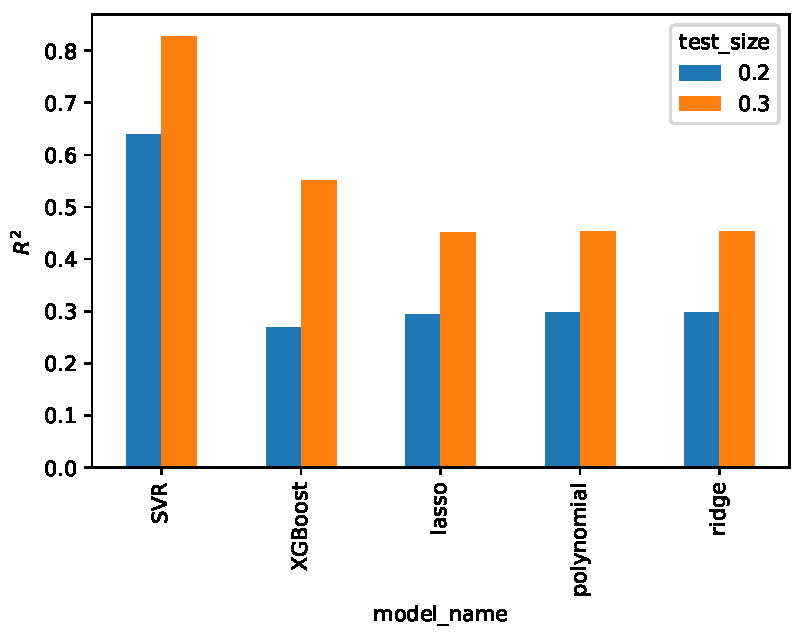
\includegraphics[width = 0.95\textwidth]{figures/test_evaluation.pdf}\end{center}
\vspace{-0.7cm}
\caption{Evaluation of the fitted models accuracy}
\label{fig:test_evaluation}
\end{figure}
\begin{figure}[H]
\begin{center}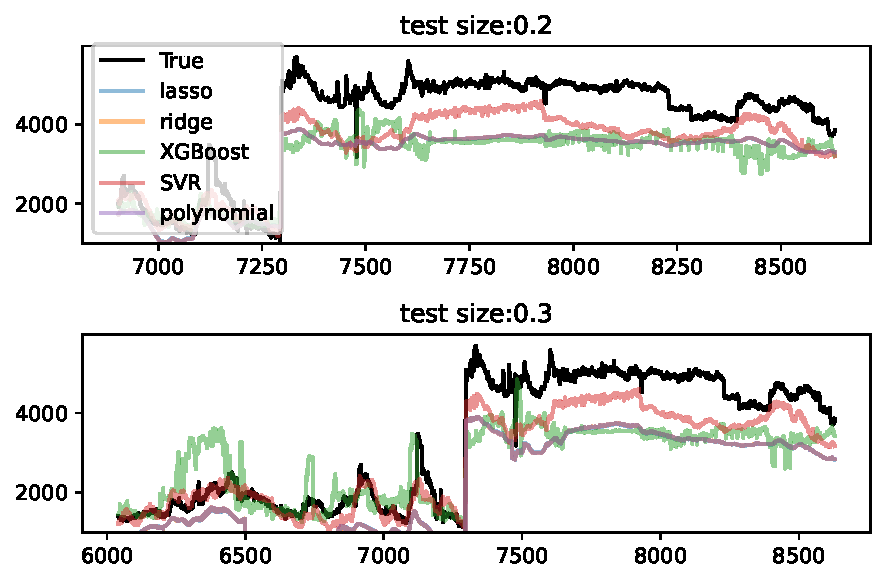
\includegraphics[width = 0.95\textwidth]{figures/predictions.pdf}\end{center}
\vspace{-0.7cm}
\caption{Predictions on the test data sets}
\label{fig:predictions}
\end{figure}
\begin{equation}
y = - 944.923049 T + 244.319815 U_{wind} + 2964.727832
\label{eq:model_polynomial}
\end{equation}
